\section{Introduction to Fusion}
\begin{frame}{Fusion Reactions}
	There are a few fusion reactions,
	\begin{itemize}
		\item D-T reaction: large cross-section at low temperature, but hard to find Tritium.
		      \[ ^2_1D + ^2_1T \rightarrow ^4_2He + ^1_0n + 17.6\text{MeV} \]
		\item D-D reaction: easy to find the fuel, but small cross-section at low temperature.
		      \[ ^2D + ^2D \rightarrow ^3He + ^1n + 3.27\text{MeV} \]
		      \[ ^2D + ^2D \rightarrow ^3T + 4.03\text{MeV} \]
		\item D-He reaction: easy to find the fuel, but small cross-section at low temperature.
		      \[ ^2D + ^3He \rightarrow ^4He + ^1H + 18.3\text{MeV} \]
	\end{itemize}
\end{frame}

\begin{frame}{Cross-section}
	\begin{figure}
		\centering
		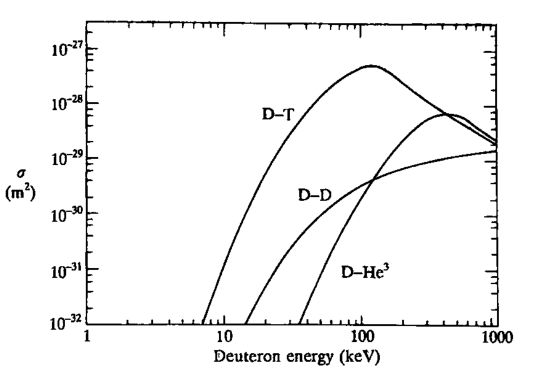
\includegraphics[width=0.7\textwidth]{figures/cross-sections.png}
		\caption{Adapted from \cite{wesson_campbell_tokamaks_2011} Cross-sections for the reactions D-T, D-D and D-$^3$He. The two D-D reactions have similar cross-sections, the graph gives their sum. At 100keV, D-T reaction has the largest cross-section, meaning that more fusion reactions happen in D-T reaction compare to the other two reactions.}
		\label{fig:cross-sections}
	\end{figure}
\end{frame}

\begin{frame}{Thermonuclear Fusion}
	The reaction rate is given by
	\begin{equation}
		R = \left(\frac{8}{\pi}\right)^{1/2}n_1n_2\left(\frac{\mu}{T}\right)^{3/2}\frac{1}{m_1^2}\int \sigma(\epsilon)\epsilon\exp(-\frac{\mu\epsilon}{m_1T})d\epsilon
		\label{eq:reaction-rate}
	\end{equation}
	where the subscript 1 and 2 are D and T, respectively. And $n$ is the number density, $\mu=m_1m_2/(m_1+m_2)$ is the reduced mass, and $\epsilon=\frac{1}{2}m_1(v_1-v-2)^2$ is the kinetic energy of D.
	\begin{itemize}
		\item The rate is maximized when $n_1=n_2$.
		\item The cross-section $\sigma$ is given by Fig.\ref{fig:cross-sections}.
	\end{itemize}
\end{frame}

\begin{frame}{$\expval{\sigma v}$}
	\begin{figure}
		\centering
		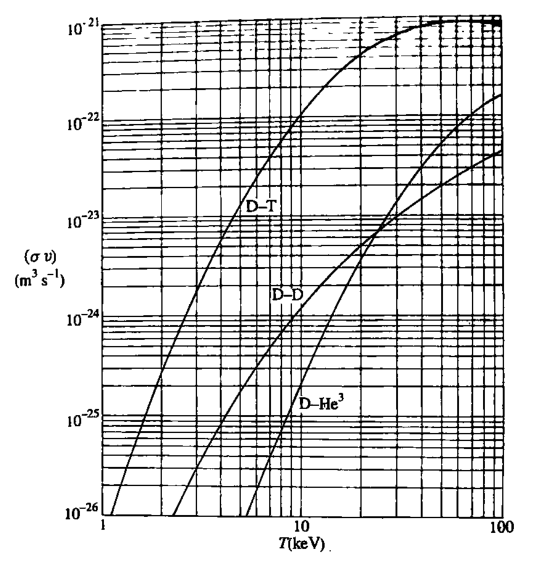
\includegraphics[width=0.4\textwidth]{figures/sigma-v.png}
		\caption{Adapted from \cite{wesson_campbell_tokamaks_2011}, $\expval{\sigma v}$ for D-T, D-D(total) and D-$^3$He reactions as a function of plasma temperature. $\expval{\sigma v}$ for D-D and D-$^3$He are much smaller than that of D-T.}
		\label{fig:sigma-v}
	\end{figure}
\end{frame}